\section{Introduction}
\label{sec:intro}

Online user review is an essential part of e-commerce. 
Popular e-commerce websites feature enormous amount of text reviews, especially for popular products and services. 
To improve the user experience and expedite the
shopping process, many websites provide either qualitative or quantitative
summary of user reviews, typically organized by important aspects or characteristics.
For example, \figref{fig:tripadvisor} shows a short review passage from a customer on TripAdvisor.com, and the customer is also asked
to give discrete ratings on several specific aspects of 
the hotel, such as location and cleanness. 
%This kind of ratings from individual reviews can then be aggregated into an overall
%ratings from many users.
%Aggregation from this kind of individual ratings can be beneficial  
Such review summarization with specific aspects is defined as \emph{aspect-based review 
	summarization}~\cite{hu2004mining}, which more efficiently represents the customer feedback and thus is desired by both sellers and potential customers.

With aspect-based reviews summarization, potential customers can touch more details with various aspects of a product directly. 
They do not have to read a large amount of reviews and then make an evaluation considering different dimensions by themselves.
Also,   
aspect-based review summarization provides an effective and efficient way for 
comparing similar products from different brands, since they share 
the same review aspects and then can be compared with each other in multiple dimensions.
At present, aspect-based review summary offered by e-commerce typically 
falls into two main types: 
1) manually created aspects and 2) automatically mined product-specific phrase sets.
We discuss these two types in the following two paragraphs.
% such as those shown
%about a specific car model in \figref{fig:cars.com}, a snapshot from Cars.com. 
%Aspect-based review summarization is commonly seen on websites 
%like TripAdvisor and Cars.com. 

%Aspect-based reviews have several advantages compared to the more traditional 
%style of online reviews that consists of a short passage and an overall rating. 



%\begin{figure}[th]
%\centering
%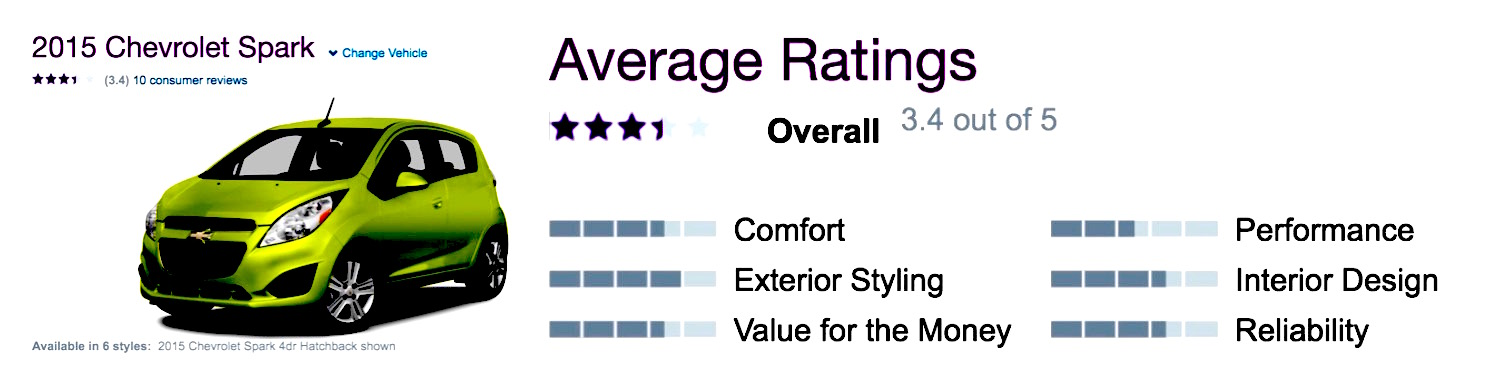
\includegraphics[width=1.0\columnwidth]{figures/cars}
%\caption{Review summarization from Cars.com.}
%\label{fig:cars.com}
%\end{figure}

Some websites that only sell (or review) a very small number of products and services tend to manually select the aspects of their target products.
For example, TripAdvisor.com only features travel-related products, and Cars.com only reviews automobiles. 
It is true that in-depth knowledge from human is the best way of
characterizing a product type with a few keywords
and the desired size of aspect terms are indeed small enough for human to manually choose them.
Nonetheless, as for many popular general  e-commerce platforms, such as Amazon, ebay,  Taobao and Yelp, 
there are a large amount of product types.
Plus, new product types and service types are emerging almost everyday. 
Therefore, human labor would be too expensive and impractical to attack this task and it can also be difficult for human to predefine aspect terms for some emerging products. The key aspects of a product may also change in time.
For example, in the past, people care more about the screen size and picture
resolution of cell phones. These are no longer issues in present days. People
instead turn to issues such as battery life and processing speed, etc.
%\BL{better have an example of emerging product}

\begin{figure}[th!]
	\centering
	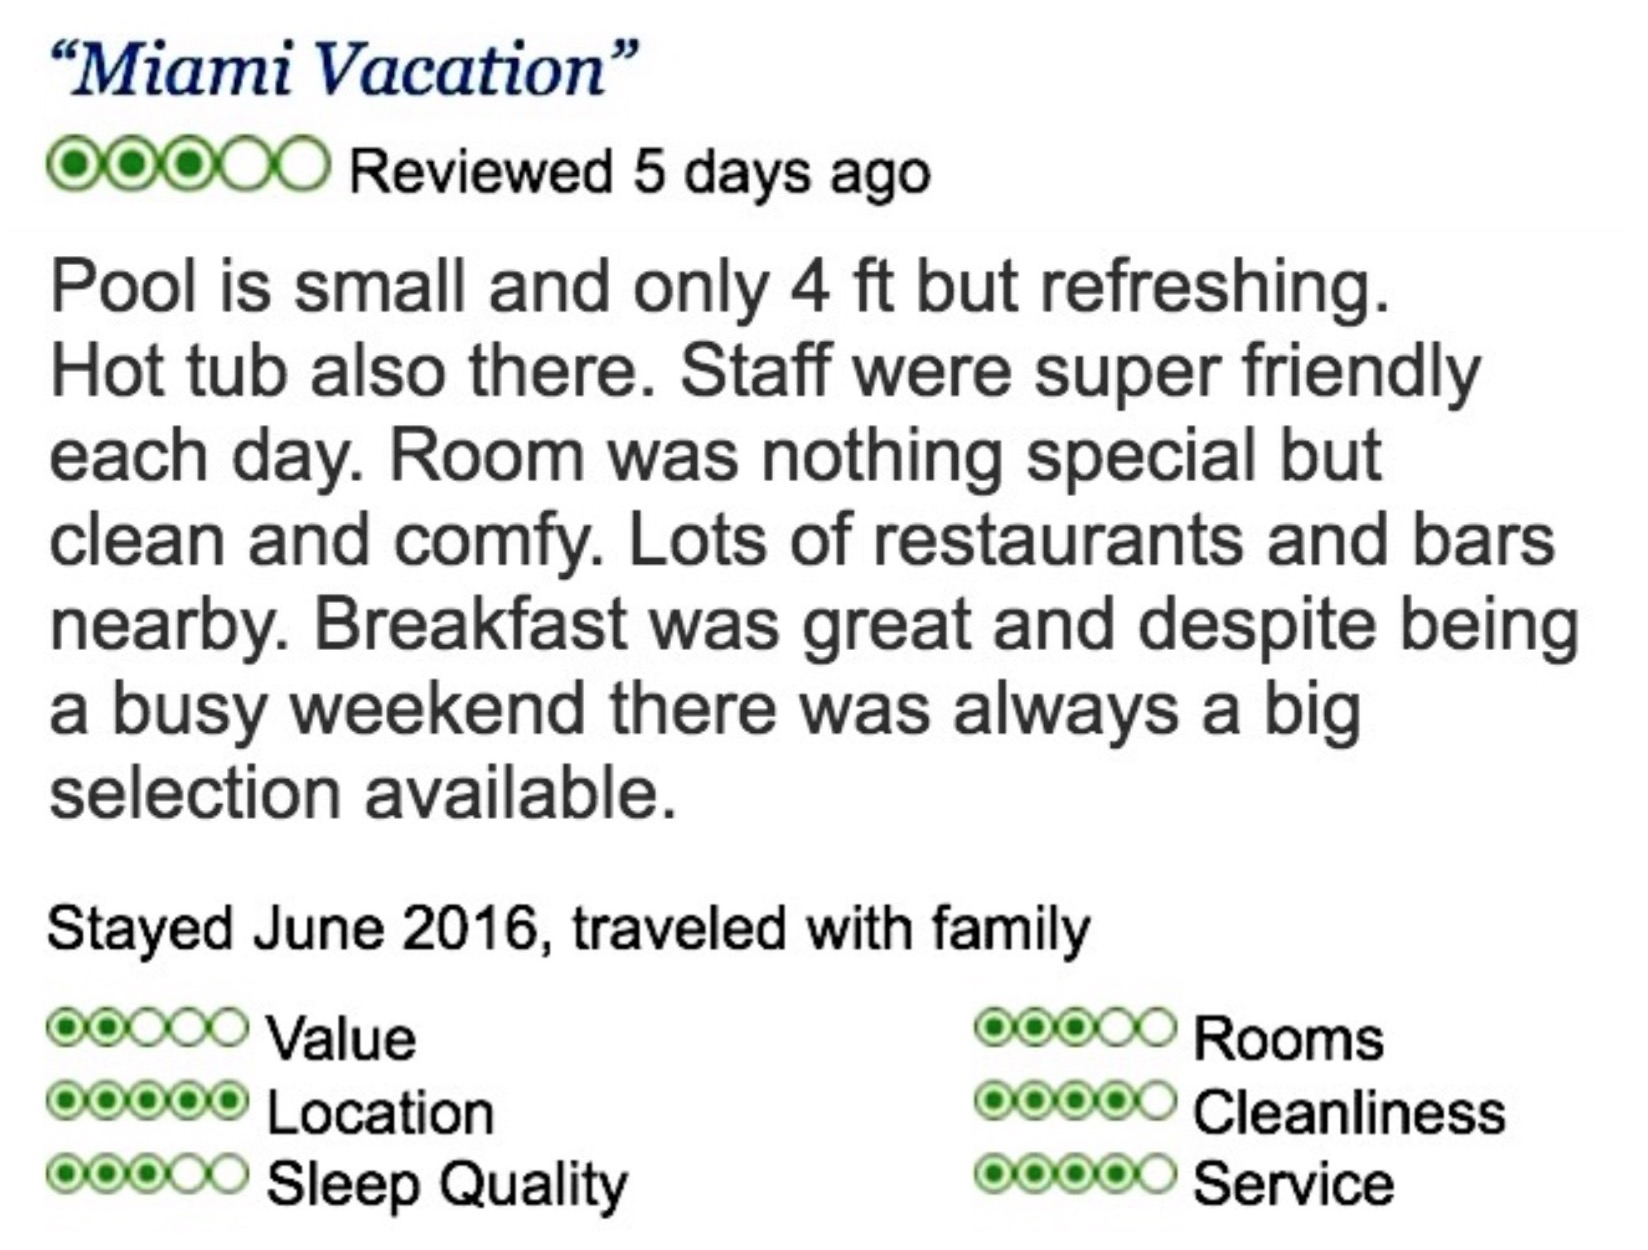
\includegraphics[width=0.7\columnwidth]{figures/tripadvisor}
	\caption{User review from TripAdvisor.}
	\label{fig:tripadvisor}
\end{figure}
%
%Manual selection of aspects 
%certainly cannot scale to such large number of
%product types. 
%These platforms instead turn to automatic review 
%summarization, mined from the user review texts. 

In general e-commerce websites, a common example of automatic review summarization 
is shown in \figref{fig:phrases}. 
There are a set of automatically mined phrases for each phone model, 
along with the frequency of each phrase mentioned in the 
reviews. 
However, there are two drawbacks in this form of summarization:
1) the set of phrases are from reviews of a specific product, and thus 
summaries appear to be different across different products within 
the same category, which makes comparison between products on a set of shared
features difficult and unintuitive;
2) the emotional terms in the phrases would cause that potential customers cannot computationally see a broader level of reviews or computationally compare different products.

\begin{figure}[th]
\centering
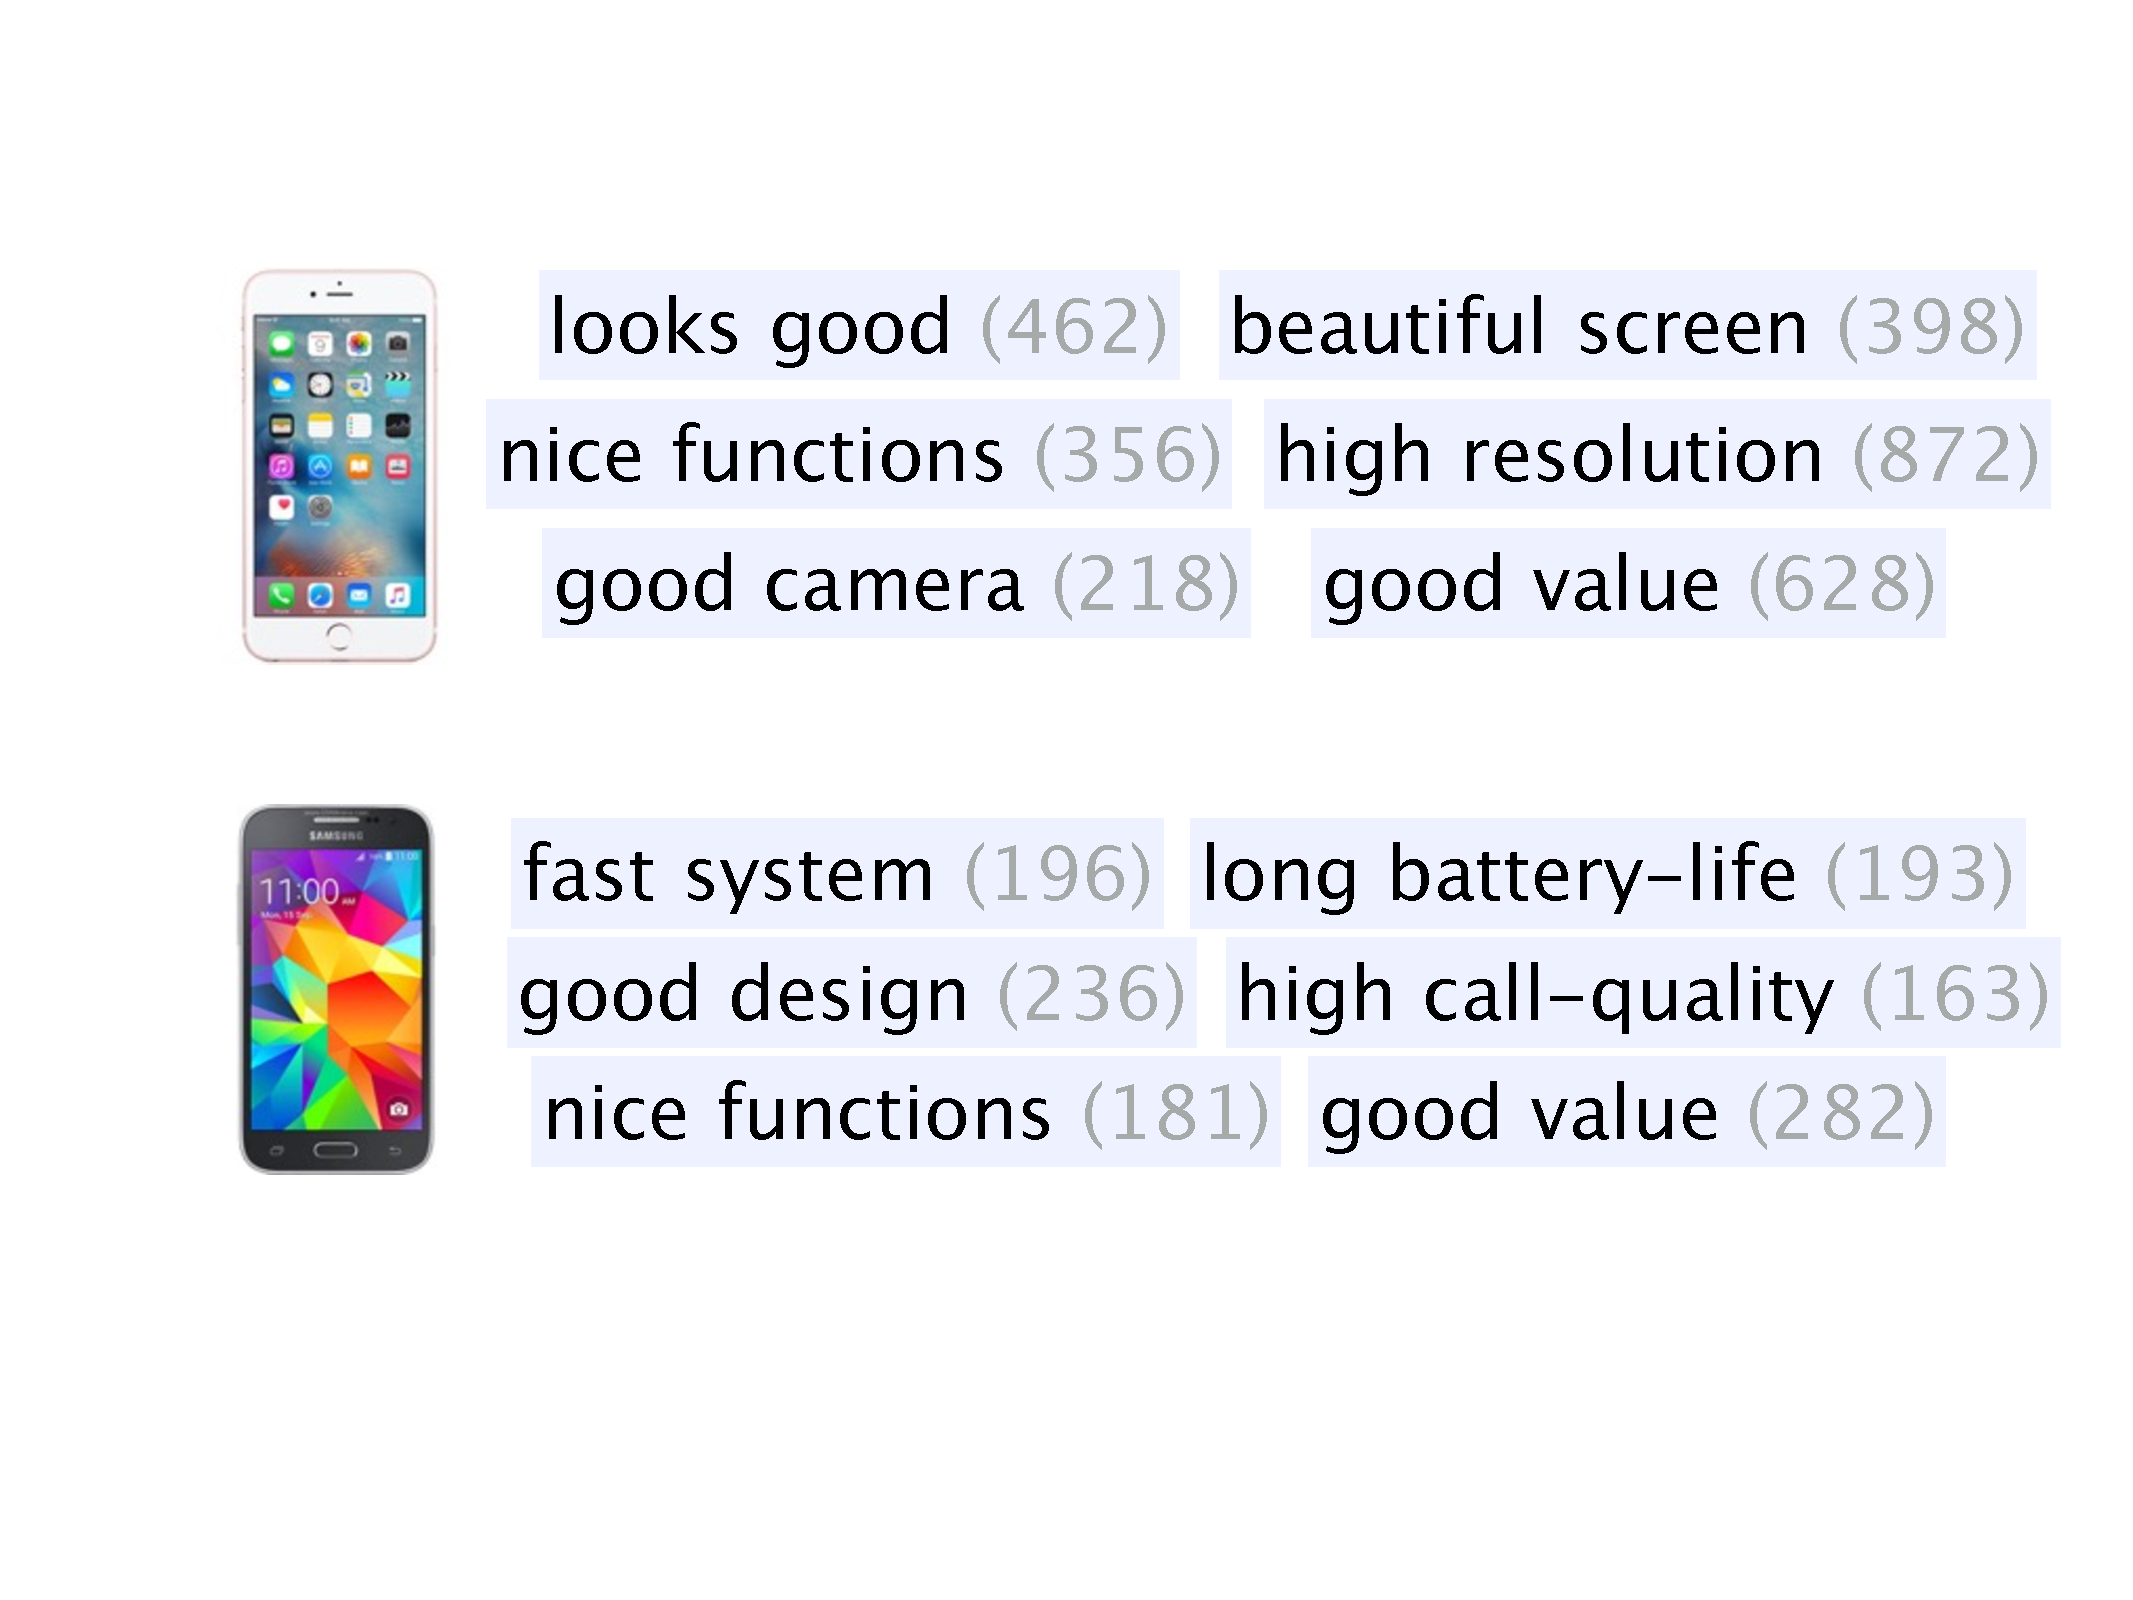
\includegraphics[width=0.6\columnwidth]{figures/phrases}
\caption{Automatic review summarization for two mobile phones 
	on an e-commerce website}
\label{fig:phrases}
\end{figure}

%3) this method can only apply on 
% user cannot choose to express them differently.

%The aspects of a product are supposed to capture the most important features 
%and cover all the facets of the product. The products of the same category 
%share the same set of aspects, however the aspects can be very different 
%across categories. It takes both common knowledge and personal experience 
%with the product to decide which are the appropriate aspects. 
%The websites that can provide aspect-based rating system basically 
%all share a common feature, that is they each focuses on only one or 
%a small range of products. For example TripAdvisor focuses on hotels and 
%Cars.com focuese on cars. The set of aspects is what the consumers base 
%on to compare different products, thus they must be carefully chosen 
%to cover all the facest of the product. Moreoever, at the end of the day 
%the aspects is designed to serve the consumers, especially potential consumers, 
%so they need to reflect what the consumers care about the product. 
%Ideally, the aspects should be decided with user reviews taken into 
%consideration. For a small range of products, the website owner or 
%the retailer may manual designate the set of aspects, 
%however this is intractable for websites like Amazon and TaoBao, 
%which host basically all kinds of products available on the market, 
%and websites like Yelp on which users review thousands of different services. 
%
%Motivated by this observation, we are in need for methods that automatically 
%generate review summarizations. 

Our goal in this paper is to develop an unsupervised framework 
for automatically extracting review aspects from user review corpora for any given product type.  
%The formulation of aspects extraction, 
%which is extracting words from a set of documents, 
%is similar to topic modeling where aspects can be seen as topics. 
%While the task seems to be similar with topic modeling on the a set of review documents,
There are three main factors that make review aspect extraction 
more challenging:
\begin{itemize}
    \item 
	In aspect extraction, we expect the final 
	aspect words to have little semantic overlaps with each other, 
	so as to avoid very general and vague terms.
    \item The expression of opinions can be very versatile. 
          In user reviews, aspects can appear both explicitly by 
	direct references or through users' personal experiences implicitly.
    \item It is very common that opinions about multiple aspects are stated within a very short piece of comment, so the topics may shift from sentence to sentence much faster than other short documents.
\end{itemize}

Most previously proposed unsupervised approaches for aspect extraction are 
variations of topic modeling techniques. 
The main problem with topic-model-based methods 
is they typically leverage only word frequencies and co-occurrences information instead of semantics, 
and thus they cannot effectively detect the sentences that are superficially different but semantically talking about similar aspects. 
%\BL{Jessie please describe our framework briefly here, using similar words in the following sections} 

In our framework, ExtRA, we perform topic modeling on sentence clusters to generate potential aspect topics, and cluster the potential topics to obtain the final pured aspect clusters. 
We design two ranking metrics respectively for pruning aspect clusters and ranking candidate aspect terms, 
in which we represent aspect clusters with vectors (AspVec) in a shared space with aspect terms.
%with aspect candidates benefiting from our ranking mechanism. 
Finally, our framework can then extract aspect words and phrases by simply computing the similarities between each AspVec and all the candidate aspect terms (words or phrases).

%we leverage the distributed 
%representations of words and sentences, which help us first cluster the similar sentences.
%With distributed representations, 
%the semantic similarity between two sentences can be more accurately 
%calculated without relying too much on the lexical information.
%Our proposed method consists 3 clustering steps and
%2 ranking phase. 

Our work has four main contributions:

\begin{enumerate}
    \item We proposed a novel unsupervised framework for aspect extraction from customer review corpus about any given product or service type. 
    \item Extensive experiments showed that our framework is effective and outperforms the state-of-the-art methods.
    \item We open-sourced a tool of our framework\footnote{Our tool is available at \url{http://anonymized.due.to.blind.review}}  and an evaluation dataset for future aspect extraction research.
    \item We also built a demo website\footnote{Our demo website is available at \url{http://anonymized.due.to.blind.review}} for visualizing the mined review aspects and their potential applications.
\end{enumerate}

In \secref{sec:method} we introduce our framework ExtRA step-by-step.
Then, in \secref{sec:experiments} we evaluate our framework on multiple domains, demonstrate 
the effectiveness of our model against other approaches 
and show how the extracted aspects can be used
to construct a complete review summarization. 
Finally, in \secref{sec:related}, we discuss
and compare our work with previous research on aspect-based review 
summarization.

